% !TEX root =  master.tex
\chapter{Analyse und Bewertung von Poolingmethoden}
Auf der Evaluierung der Poolingmethoden wurden mathematisch sinnvolle Verfahren für die jeweiligen Inzidenzstufen ermittelt.
Diese sollen nun um weitere Parameter erweitert werden, um ihre Tauglichkeit im betrieblichen Umfeld zu ermitteln.

\section{Eindimensionales Pooling}
Begonnen wird mit einem einfachen, eindimensionalen Poolingverfahren als spätere Referenz.
Kompliziertere Verfahren werden später erläutert um zu prüfen, ob hierdurch ein Mehrwert beobachtet werden kann.
Hierdurch wird sichergestellt, dass das einfachstmögliche Verfahren angewandt wird.
Umfangreiche Methoden werden nur weiter verfolgt, wenn sie das einfache Referenzverfahren übertreffen.

Das einfachste Verfahren für Pooling ist, eine eindimensionale Reihe von Proben zu verwenden und diese vor der PCR-Analyse zu kombinieren.
Die Matrix lässt sich hierbei als 1xN beschreiben.
Die Proben werden gemeinsam getestet.

\subsubsection{Effizienzkurve Eindimensionale Pools}
Für das eindimensionale Poolingverfahren ergibt sich insgesamt die folgende Effizienzkurve.

Eine vollständige gegenüberstellung in tabellarischer Form ist im Anhang dargestellt.
\begin{figure}[h]
	\centering
	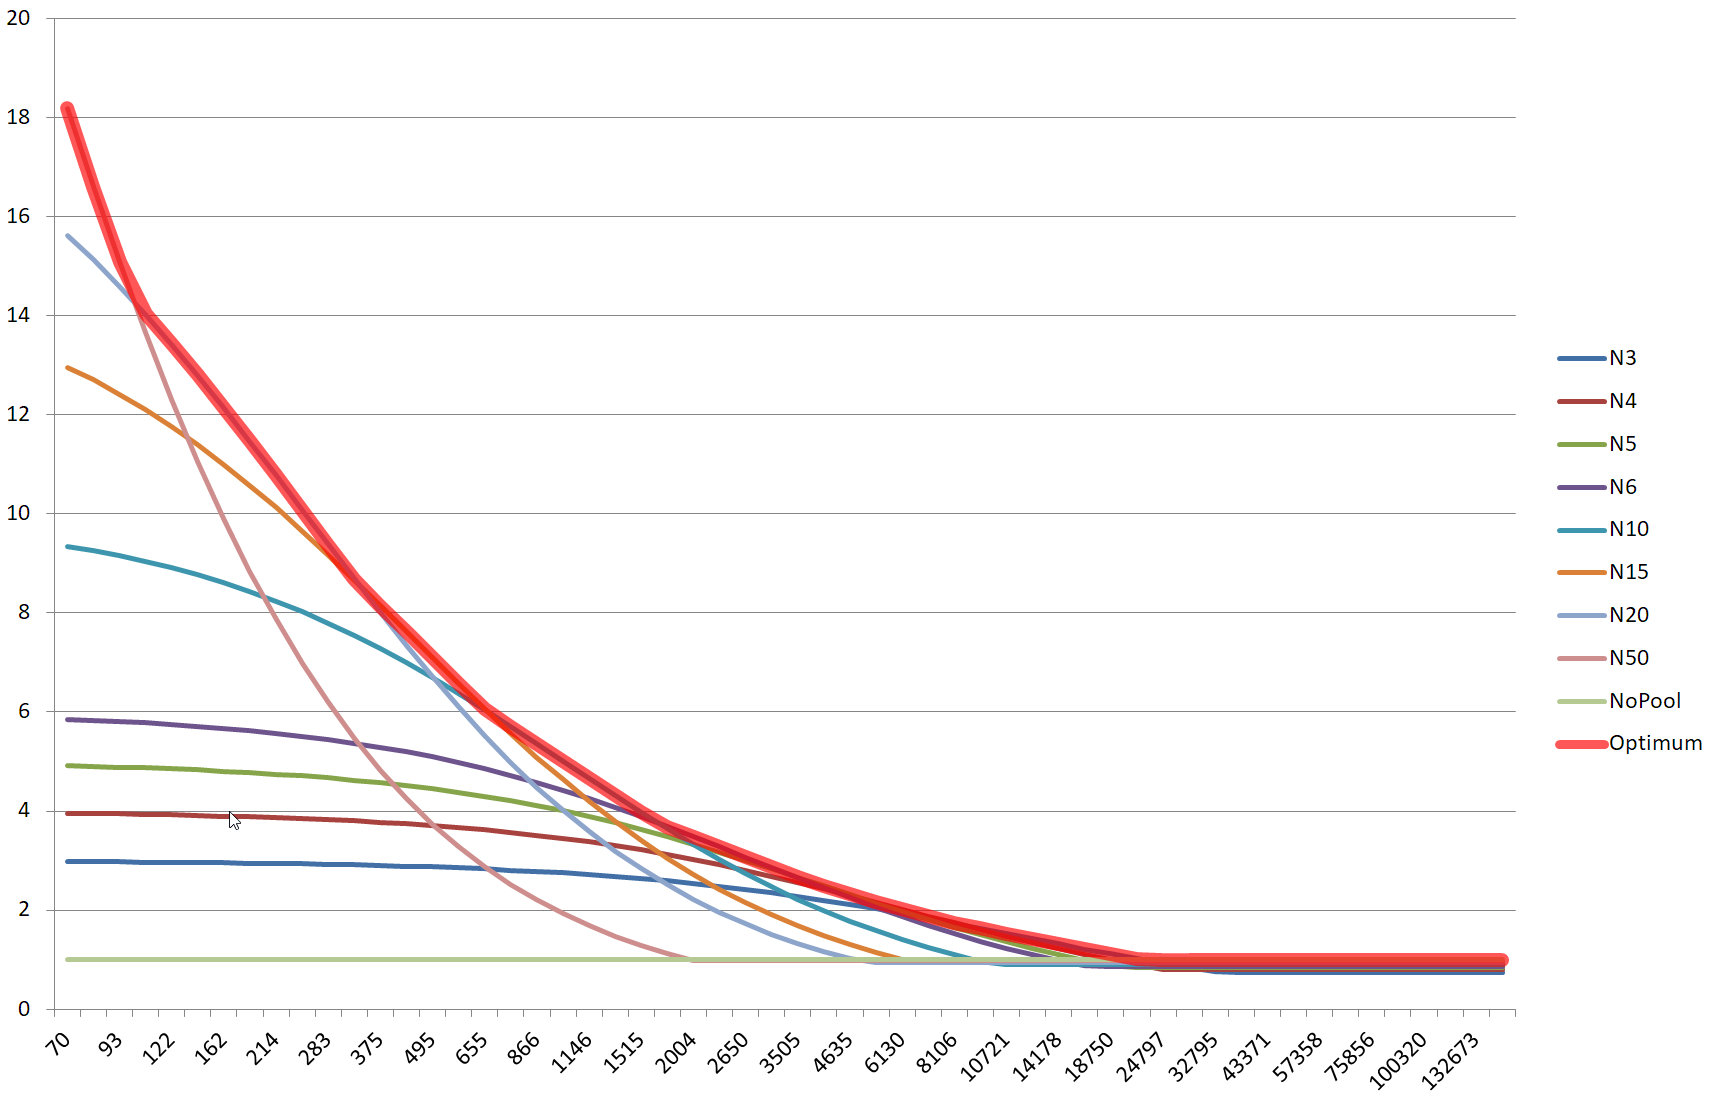
\includegraphics[height=.6\textwidth]{img/1D_Pool-EffKurve}
	\caption{Effizienzkurve des eindimensionalen Poolingverfahrens\footnotemark}
\end{figure}

Als logarithmische Tabelle bedeutet dies:

\begin{tabular}{|c|c|}
	\hline
	Prävalenz (von 100.000) & Erwartungswert \\
	\hline
	1 & sdf \\
	\hline
	10 & sdf \\
	\hline
	100 & asdad \\
	\hline
	1.000 & sdfsd \\
	\hline
	10.000 & dfg \\
	\hline
	100.000 & dfg \\
	\hline
\end{tabular}

\cleardoublepage

\section{Zweidimensionales Pooling}
Bei dieser Poolingmethode handelt es sich um einen zweidimensionalen Pool, mit dem Ziel, den Bedarf einer Nachtestung bei einzelnen Positivfällen zu minimieren.
Die Testpersonen werden in einer AxB-Matrix angeordnet.
Die Proben werden dann für jede Spalte und jede Reihe gepoolt.
Allgemein formuliert lässt sich sagen:
Testbedarf pro Person =
$\frac{A+B}{A\cdot B}$

Die Testgruppe lässt sich geometrisch als Rechteck beschreiben.
Die Kanten A und B ergeben in Summe die benötigte Testanzahl.
Die Fläche beschreibt die mögliche Anzahl der zu testenden Personen.
Aus der Geometrie ist bekannt,\footnote{Geometrie Quadrat}
dass das Verhältnis von Fläche zu Kantenlänge bei einem Quadrat optimal ist.
Bei dieser Methode kommen somit nur Quardate als effizient infrage.
Hierdurch lässt sich festlegen, dass $A=B$.

Für eine Testgruppe von 25 Personen, welche in einer 5x5 Matrix angeordnet sind, werden somit 5+5 Tests benötigt.
Die Effizienz läge bei 2,5 Personen pro Test.
Vergleichen mit dem eindimensionalen Poolingverfahren klingt das zunächst nicht nach sehr viel.
Allerdings ist dieses Verfahren darauf optimiert, robust gegen einzelne Positivfälle zu sein.
Die Hypothese wäre somit, dass es bei hohen Prävalenzen einen Vorteil bietet, da nicht alle Testpersonen erneut getestet werden müssen.

Die Wahrscheinlichkeit, dass der Pool positiv ist verändert sich zum anderen Testverfahren nicht.
Sie hängt wieder von Prävalenz und Größe der Testgruppe ab.
Deshalb gilt weiterhin:
P(PoolPositiv) = $(min\left(1;Poolsize\cdot Pravalenz\right)$

Bei der Nachtestung im Falle eines positiven Pools werden allerdings nicht mehr alle Personen nachgetestet.
Sollte nur eine Person in der Testgruppe positiv sein, so kann dessen Position in der Testgruppe anhand der positiven Pools abgelesen werden.
\begin{figure}[h]
	\centering
	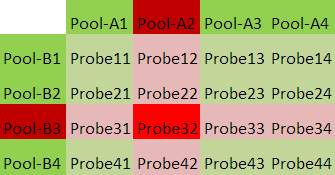
\includegraphics[height=.25\textwidth]{img/2d_Pool_1Positiv}
	\caption{Zweidimensionaler Pool mit einer positiven Person (Probe32). Die Pools A2 und B3 werden positiv und weisen auf die Position 3-2 der positiven Probe. Für die Hellrot unterlegten Personen liegt ein positiver und ein Negativer Pool vor.\footnotemark}
\end{figure}

Erwartungswert Personen pro Test =
%$\frac{A\cdot A} {P(PoolPositiv)\cdot (Poolsize + 1)) + (1 - P(PoolPositiv))}$

Die beiden positiven Personen (1-4 und 3-2) in Abb 3.3 lösen die Tests A2, A4, B1 und B3 aus.
Neben den positiven Personen zeigen diese Tests auch auf die eigentlich negativen Proben 1-2 und 3-4.
Aus diesem Grund müssen hier für zwei positive Personen vier Proben nachgetestet werden.

Grundsätzlich verhält sich der Bedarf an Nachtestungen quadratisch zur Anzahl der Positiven Personen.
Es ist allerdings möglich, dass mehrere positive Personen in einem Test sind.
Durch diese Überschneidung verringert sich der Bedarf für Nachtestungen, weswegen eine Clusterung positiver Tests vorteilhaft sein kann.

\cleardoublepage
\section{Viehweger}
Bei Poolgröße 20 und 2 Prozent Prävalenz Erreicht diese Methode eine Effizienzsteigerung um den Faktor 5.\footnote{Viehweger Z14}


%\section{Blutspendedienste}
In Deutschland haben die größte Erfahrung die Blutspendedieste zu haben, da diese seit Jahrzehnten Pooling-Verfahren einsetzen um auf HIV und Hepatitis zu testen (Ärtzeblatt). Diese haben hierfür auch ein Patent angemeldet. Die Methode dieses Patents soll die Basis für den Vergleich anderer Verfahren sein.

%\section{Forschungsgruppe 3}

%\cleardoublepage


%#########################################################
%#########################################################
\if{false}
\section{Planung aus RP}
Die Beantwortung der primären Forschungsfrage beginnt mit einer Aufbereitung der bisherigen Forschung zu PCR-Pooling-Verfahren.
Für die Validierung sind zwei Forschungsansätze denkbar:

Qualitativer Ansatz:
Die Disziplin der Kanalcodierung wird vorgestellt und auf Basis dieses wissenschaftlichen Frameworks die Pooling-Verfahren formalisiert.
Hierauf erfolgt eine argumentativ-deduktive Analyse, welche die Methode durch theoretische und qualitative Ansätze überprüft.


\section{Obsidian Sammlung}
\subsubsection{Kanalcodierung}
\begin{itemize}
	\item In der Raumfahrt ist Strahlung eines der Hauptprobleme, welche Bitflips
	\footnote{Die binäre Änderung eines Speicherfeldes}
	in Speichern auslösen kann.
	Hierbei sind oftmals Fehler inakzeptabel, weswegen hochgradig redundante Systeme zum Einsatz kommen.
	Es werden Teilweise ganze Systeme mehrfach verbaut, um die Ergebnisse zu vergleichen.
	\item Ethernetpakete haben dieselbe Herausforderung wie die Raumfahrt, dass durch Störungen Bits verloren gehen können.
	Üblicherwiese sind Ethernetpakete allerdings unkritischer, können erneut gesendet werden und die Strahlungsintensität ist geringer.
	Deshalb werden hier Fehler nur erkannt, aber auf eine Korrektur verzichtet.
	Beschädigte Pakete werden verworfen und müssen erneut gesendet werden.
	\item Anhand der existierenden RAID-Level können die unterschiedlichen Ziele von Kanalcodierung veranschaulicht werden.
	Zwischen Sicherheit, Verfügbarkeit und Berechnungsintensität muss eine Abwägung getroffen werden.
	- Ein System kann wie bei RAID-0 zulasten seiner Integrität beschleunigt werden.
	- Bei RAID-1 wird wie in der Raumfahrt eine volle Redundanz hergestellt. Die hohe Fehlertoleranz der Daten wird hierbei durch hohen Mehraufwand erkauft.
	- RAID-5 und RAID-6 versuchen die Speicherkosten zu optimieren und eine dem Umstand angemessene Datensicherheit zu erreichen. Hierbei wird ein deutlicher Berechnungsaufwand für die Parität, eine lange Rebuild-Zeit und ein gewisses Ausfallrisiko in Kauf genommen.
	\item Der Reed-Solomon-Code, welcher Beispielsweise in CDs eingesetzt wird, ist in der Lage Burst-Errors
	\footnote{Fehler, welche nicht zufällig verteilt sind, sondern in Clustern auftreten.}
	zu erkennen.
	Bei CDs kann dies der Fall sein, wenn diese durch einen zusammenhängenden Kratzer beschädigt ist.
	\item Der Hamming Code war einer der ersten ECC-Algorithmen und wurde in den 1950ern von Richard W. Hamming entwickelt.
	Seine Verteilung der Paritäts-Bits ermöglicht eine effiziente Überprüfung der Daten.
	Durch Verwendung von N+1 Paritäts-Bits, kann die Integrität von 2-hoch-N Daten zu überprüfen werden.
	Die Berichtigung einzelner Bitfehler ist ebenfalls möglich.
	Sollte mehr als ein Fehler innerhalb des Blocks auftreten, kann dieser zwar erkannt, aber nicht berichtigt werden.
	Für einen Speicherbereich mit 256 Bit werden somit 8+1 Paritäts-Bits benötigt, was einem Overhead von nur 3,5 Prozent entspricht.
	Neuere Algorithmen haben die Effizient weiter gesteigert und sollen im Laufe der Arbeit vergleichen werden.
\end{itemize}

\subsubsection{Erstellung eigener Modelle}
Geprüft werden soll die Übertragbarkeit mehrerer in der Informatik gängigen ECC-Algorithmen auf den medizinischen Bereich.
Die Theorie wäre, dass Covid-Infektionen bei anlasslosen Testungen wie auch Bitfehler selten sind.
Somit könnten dieselben Algorithmen zur Effizienzsteigerung genutzt werden.
Ziel ist es, eine Möglichkeit zu finden die exponentielle Effizienzsteigerung von ECC-Algorithmen auf medizinische Testungen anzupassen und hierdurch die Kosten deutlich zu reduzieren.
Hierbei müssen Anpassungen an den Algorithmen vorgenommen werden und neue Herausforderungen beachtet werden.

Beispielsweise sind bei einem 15-11-Hamming-Code nur 11/16 Bits echte Daten.
Die Paritätsbits kosten hier direkt Speicherkapazität.
Bei einer PCR-Testung wären theoretisch alle 16 Plätze verwendbar, da die Durchführung von PCR-Tests selbst (anders als bei Speicher) keine Plätze kostet.
Desweiteren sind neue Probleme zu erwarten, wenn die Tests von Menschen durchgeführt werden.
Hierbei entstehen Fehler, welche in den bisherigen Algorithmen keine Berücksichtigung finden mussten.


\section{Planung aus RP - Quant}
Die Beantwortung der primären Forschungsfrage beginnt mit einer Aufbereitung der bisherigen Forschung zu PCR-Pooling-Verfahren.
Für die Validierung sind zwei Forschungsansätze denkbar:

Quantitativer Ansatz:
Die Pooling-Verfahren werden in Software nachgebaut und quantitativ anhand einer Simulation analysiert.
Es werden unterschiedliche Grenzfälle getestet, um die Auswirkung auf das Verfahren zu beobachten.


\section{Obsidian Sammlung}
\fi